\documentclass[11pt,a4paper]{article}
\usepackage[utf8]{inputenc}
\usepackage[T1]{fontenc}
\usepackage{amsfonts}
\usepackage[french]{babel}
\frenchbsetup{StandardLists=true} % à inclure si on utilise \usepackage[francais]{babel}
\usepackage{enumitem}
\usepackage{amssymb}
\usepackage{amsmath}
\usepackage[left=2cm,right=2cm,top=2cm,bottom=2cm]{geometry}
\usepackage{multirow}
\usepackage[dvipsnames]{xcolor}

\usepackage[T1]{fontenc}
\usepackage{graphicx}
\usepackage{tikz}
\usetikzlibrary{patterns}

\usepackage{setspace}
\singlespacing

\usepackage{pstricks}
\usepackage{xkeyval}
\usepackage{pst-labo}


\usepackage{multicol}
\usepackage{caption}
\usepackage{fancyhdr}
\pagestyle{fancy}
\renewcommand\headrulewidth{1pt}
\fancyhead[L]{Lycée Denis Diderot }
\fancyhead[R]{Classe de 1 Bac Pro }
\setcounter{page}{1}\fancyfoot[C]{page \thepage}
\fancyfoot[R]{Année 2025-2026}
\fancyfoot[L]{Alexis RUIZ}
\usepackage{multirow,tabularx,booktabs}
\usepackage[tikz]{bclogo} 

\newcommand{\cadreblanc}[1]{%
\medskip\framebox[\linewidth][c]{%
\rule{0mm}{#1mm}}\par
\medskip}

\usepackage{awesomebox}
\setlength{\aweboxvskip}{0mm}
\usepackage{pifont}
\usepackage{chemmacros}
\chemsetup{modules=all}
\setlength{\columnseprule}{.25mm}

\renewcommand{\arraystretch}{1.5}
\newcommand*\acocher{\quitvmode{\fboxsep0pt \fboxrule0.8pt \fbox{\vrule height1.8ex depth.1ex width0pt \vrule height0pt depth0pt width1.9ex }}}

\newcolumntype{C}[1]{>{\centering\arraybackslash }b{#1}}

\newcommand{\code}{\awesomebox[black]{2pt}{

\includegraphics[scale=0.15]{../Chapitre 1 - Energie et puissance électrique/images/frame.png}
}{black}}

\newcommand{\moteur}{\awesomebox[black]{2pt}{

\includegraphics[scale=1]{images/moteur.jpg} 
}{black}}

\newcommand{\defbox}{\awesomebox[black]{2pt}{
\includegraphics[scale=0.5]{../Chapitre 1 - Energie et puissance électrique/images/appel exam.png}}{black}}

\newcommand{\defconclusion}{\awesomebox[black]{2pt}{\rotatebox{90}{\Large{\textbf{Conclusion}}}}{black}}

  \newenvironment{itemize*}%  % listes compactes
    {\begin{itemize}%
      \setlength{\itemsep}{0pt}%
      \setlength{\parskip}{0pt}}%
    {\end{itemize}}

\frenchbsetup{StandardLists=true}



\begin{document}


\flushleft \textbf{NOM : \hfill Classe : \hspace{3cm} ~~\\[2mm]
Prénom:\\[0,4cm]
}
\hrule\
\\[0,2cm]

\begin{center}
 \LARGE{TP2 - Effet Joule}
\end{center}

\vspace{3 mm}

\normalsize

\hrule\
\\[0,2cm]
   \begin{center}
   \textbf{Le soin et la rédaction interviendront dans la notation.}
   \end{center} 

\vfill 



\fcolorbox{black}{white}{\textbf{1. Expérience}}  \\

 \begin{enumerate}[label*=1.\arabic*.]
     \item \'A l'aide du multimètre, mesurer la valeur de la résistance $R_1$ du conducteur ohmique. 

     \vspace{3mm}
     \dotfill 

     \item Réaliser le montage ci-dessous avec la résistance $R_1$: 

     
\noindent%
\begin{minipage}{.4\textwidth}%
 \begin{bclogo}[couleur=white ,  arrondi =0.1 , logo = \bcinfo, epBarre =2]{ Matériel }

\begin{itemize*}
    \item un générateur 6V CC
    \item 1 joule mètre
    \item 3 résistances 
    \item 5 fils de connexion
\end{itemize*}
\end{bclogo}

\end{minipage}%
\hfill
\begin{minipage}{.5\textwidth}%
\begin{center}

\begin{tikzpicture}[scale=1.5, thick]

% Partie haute du circuit - générateur
% Coin supérieur gauche
\draw (0,4) -- (2.1,4);

% Générateur (cercle avec G) - rayon 0.4
\draw (2.50,4) circle (0.4);
\node[font=\Large\bfseries] at (2.5,4) {G};

% Petit signe - à gauche du cercle (0.5cm plus haut)
\node[font=\small] at (2,4.3) {$-$};

% Petit signe + à droite du cercle (0.5cm plus haut)
\node[font=\small] at (3,4.3) {$+$};

% Connexion à droite du générateur
\draw (2.9,4) -- (4.5,4);

% Fil droit qui descend
\draw (4.5,4) -- (4.5,0.5) -- (3.4,0.5);

% Coin supérieur gauche descend
\draw (0,4) -- (0,1.75);

%connection U
\draw (0.3,1.75) -- (0.3,0.5) -- (1.80,0.5);

\draw(1.8,0.8) -- (1.5,0.8) -- (1.5,1.75) ; 

% Connexion Ampèremetre
\draw (0,1.75) -- (4,1.75) -- (4,0.8) -- (3.4,0.8);

% Joulemètre - boîte rectangulaire marron (80% de largeur)
\draw[fill=blue!20] (1.8,0.0) rectangle (3.4,1.4);

% Petit rectangle blanc à l'intérieur (afficheur)
\draw[fill=white] (2.2,0.8) rectangle (3,1.1);

% Lettre U à gauche
\node[font=\Large\bfseries] at (2.0,0.8) {U};

% Lettre I à droite
\node[font=\Large\bfseries] at (3.2,0.8) {I};

% Texte Joulemètre en bas
\node[font=\normalsize] at (2.6,0.4) {Wattmètre};

% Résistance à gauche du joulemètre (rectangle)
\draw[fill=gray!20] (0.5,1.5) rectangle (1.4,2);

\node[font=\Large\bfseries] at (1,1.72) {R};



\end{tikzpicture}
\end{center}


%dessinscanné
%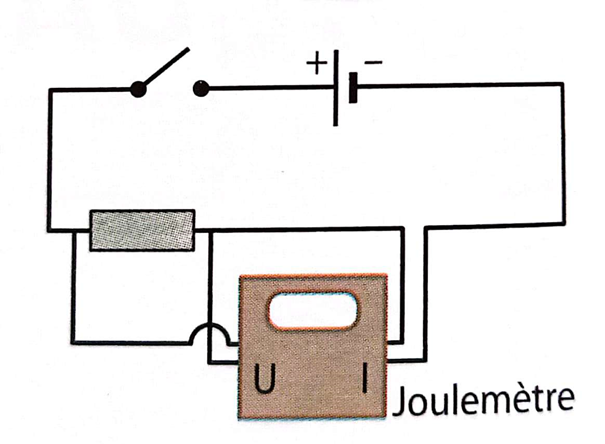
\includegraphics[width=\textwidth]{images/TP1.png}\end{center}
\end{minipage}%

\vfill 
    
\defbox{\fbox{
\begin{minipage}{8cm}{

Appeler M Ruiz pour qu'il vérifie le montage.}

\end{minipage}
}}
\item Sélectionner le mode P (puissance) et noter la valeur de la puissance P en watt consommée par le conducteur ohmique : 

\vspace{3mm}
\dotfill 

\item Sélectionner le mode U (Tension) et noter la valeur de la tension U en Volt aux bornes du conducteur ohmique : 

\vspace{3mm}
\dotfill 

\item Sélectionner le mode I (Intensité) et noter la valeur de l'intensité I en Ampère qui traverse le conducteur ohmique : 

\vspace{3mm}
\dotfill 

\item Résumer les résultats pour $R_1$ dans le tableau suivant : 

\begin{center}
    

    \begin{tabular}{|C{3cm}|C{3cm}|C{3cm}|C{3cm}|}
         \hline
         $R(\Omega)$ & $P(W)$ &  $U(V)$ & I(A) \\

         \hline
           &  &  &  \\
         \hline
 
    \end{tabular}
\end{center}




 
\vfill

\newpage 

\item \textbf{Renouveler l'expérience avec la résistance $R_2$ et écrire les résultats dans le tableau suivant} 


\begin{center}
    

    \begin{tabular}{|C{3cm}|C{3cm}|C{3cm}|C{3cm}|}
         \hline
         $R(\Omega)$ & $P(W)$ &  $U(V)$ & I(A) \\

         \hline
           &  &  &  \\
         \hline
 
    \end{tabular}
\end{center}



\item \textbf{Renouveler l'expérience avec la résistance $R_3$ et écrire les résultats dans le tableau suivant} 

\begin{center}
    

    \begin{tabular}{|C{3cm}|C{3cm}|C{3cm}|C{3cm}|}
         \hline
         $R(\Omega)$ & $P(W)$ &  $U(V)$ & I(A) \\

         \hline
           &  &  &  \\
         \hline
 
    \end{tabular}
\end{center}




\end{enumerate}




\fcolorbox{black}{white}{\textbf{2. Résultats}}  \\

 \begin{enumerate}[label*=1.\arabic*.]
 \item Recopier vos résultats dans le tableau ci-dessous 

 \item Calculer et compléter les résultats pour $\dfrac{U^2}{R}$ , $R \times I^2$ et $U \times I$ 

 
\begin{center}
    

    \begin{tabular}{|C{1.8cm}|C{1.8cm}|C{1.8cm}|C{1.8cm}||C{1.8cm}||C{1.8cm}||C{1.8cm}|}
         \hline
         $R(\Omega)$ & $P(W)$ &  $U(V)$ & I(A) & $\dfrac{U^2}{R}$ & $R \times I^2$ & $U \times I$ \\

         \hline
           &  &  & & & &  \\
         \hline
          &  &  & & & &  \\
         \hline
          &  &  & & & &  \\
         \hline
 
    \end{tabular}
\end{center}

\item Comparer les valeurs numériques de $\dfrac{U^2}{R}$ , $R \times I^2$ et $U \times I$ 

\vspace{3mm}
\dotfill 


\end{enumerate}


\fcolorbox{black}{white}{\textbf{3. Interprétation}}  \\[3mm]

Compléter les phrases suivantes : 
\begin{spacing}{2}
La puissance électrique $P$ exprimée en ........... (.....) d'un conducteur ohmique de résistance $R$ exprimée en .......... (.....) et soumis à une tension $U$ exprimée en ............ (.....) est égale à : \\ \hfill ...................... \hfill ~


La puissance électrique $P$ exprimée en ........... (.....) d'un conducteur ohmique de résistance $R$ exprimée en .......... (.....) et  traversée par une intensité $I$ exprimée en ............... (...) est égale à : \\
\hfill ...................... \hfill ~

La puissance électrique $P$ exprimée en ........ (...) d'un conducteur ohmique soumis à une tension $U$ exprimée en ........ (...) et  traversée par une intensité $I$ exprimée en ............... (...) est égale à : \\
\hfill ...................... \hfill ~
\end{spacing}

\end{document}